We perform the analysis on a dataset corresponding to $187\pm7\ipb$ integrated luminosity.

Table~\ref{tab:zzselection_all} shows the number of events observed in 
data, comparing to the expected background contribution at the \zz{} 
preselection level. The background estimation was discussed at Section~\ref{sec:backgrounds}. 
Figure~\ref{fig:zz_0j_1} the distributions of key analysis variables observed in data, comparing 
to the SM expectations from simulation in the 0-jet bin final state.  

%%%%%%%%
\begin{table}[!ht]
\begin{center}
\begin{tabular} {c|c|c|cccc}
\hline
 Jet-Bin & data & all bkg. & peaking-$WZ$/$ZZ$ & $\WW$+$\ttbar+tW$ & $\dyll$ & $\Wjets$ \\
\hline
 0-Jet & X & X & X  & X & X & X\\
 1-Jet & X & X & X  & X & X & X\\
 2-Jet & X & X & X  & X & X & X \\
\hline
\hline
\end{tabular}
\caption{Expected number of signal and background events from the data-driven methods for an 
  integrated luminosity of $187\pm7\ipb$ after applying the $\ZZ$ selection requirements. 
Both statistical and systematic uncertaities are reported. }
   \label{tab:zzselection_all}
  \end{center}
\end{table}
%%%%%%%%

%%%%%%%%
\begin{figure}[!hbtp]
\begin{center}
\label{}
\subfigure[0-Jet]{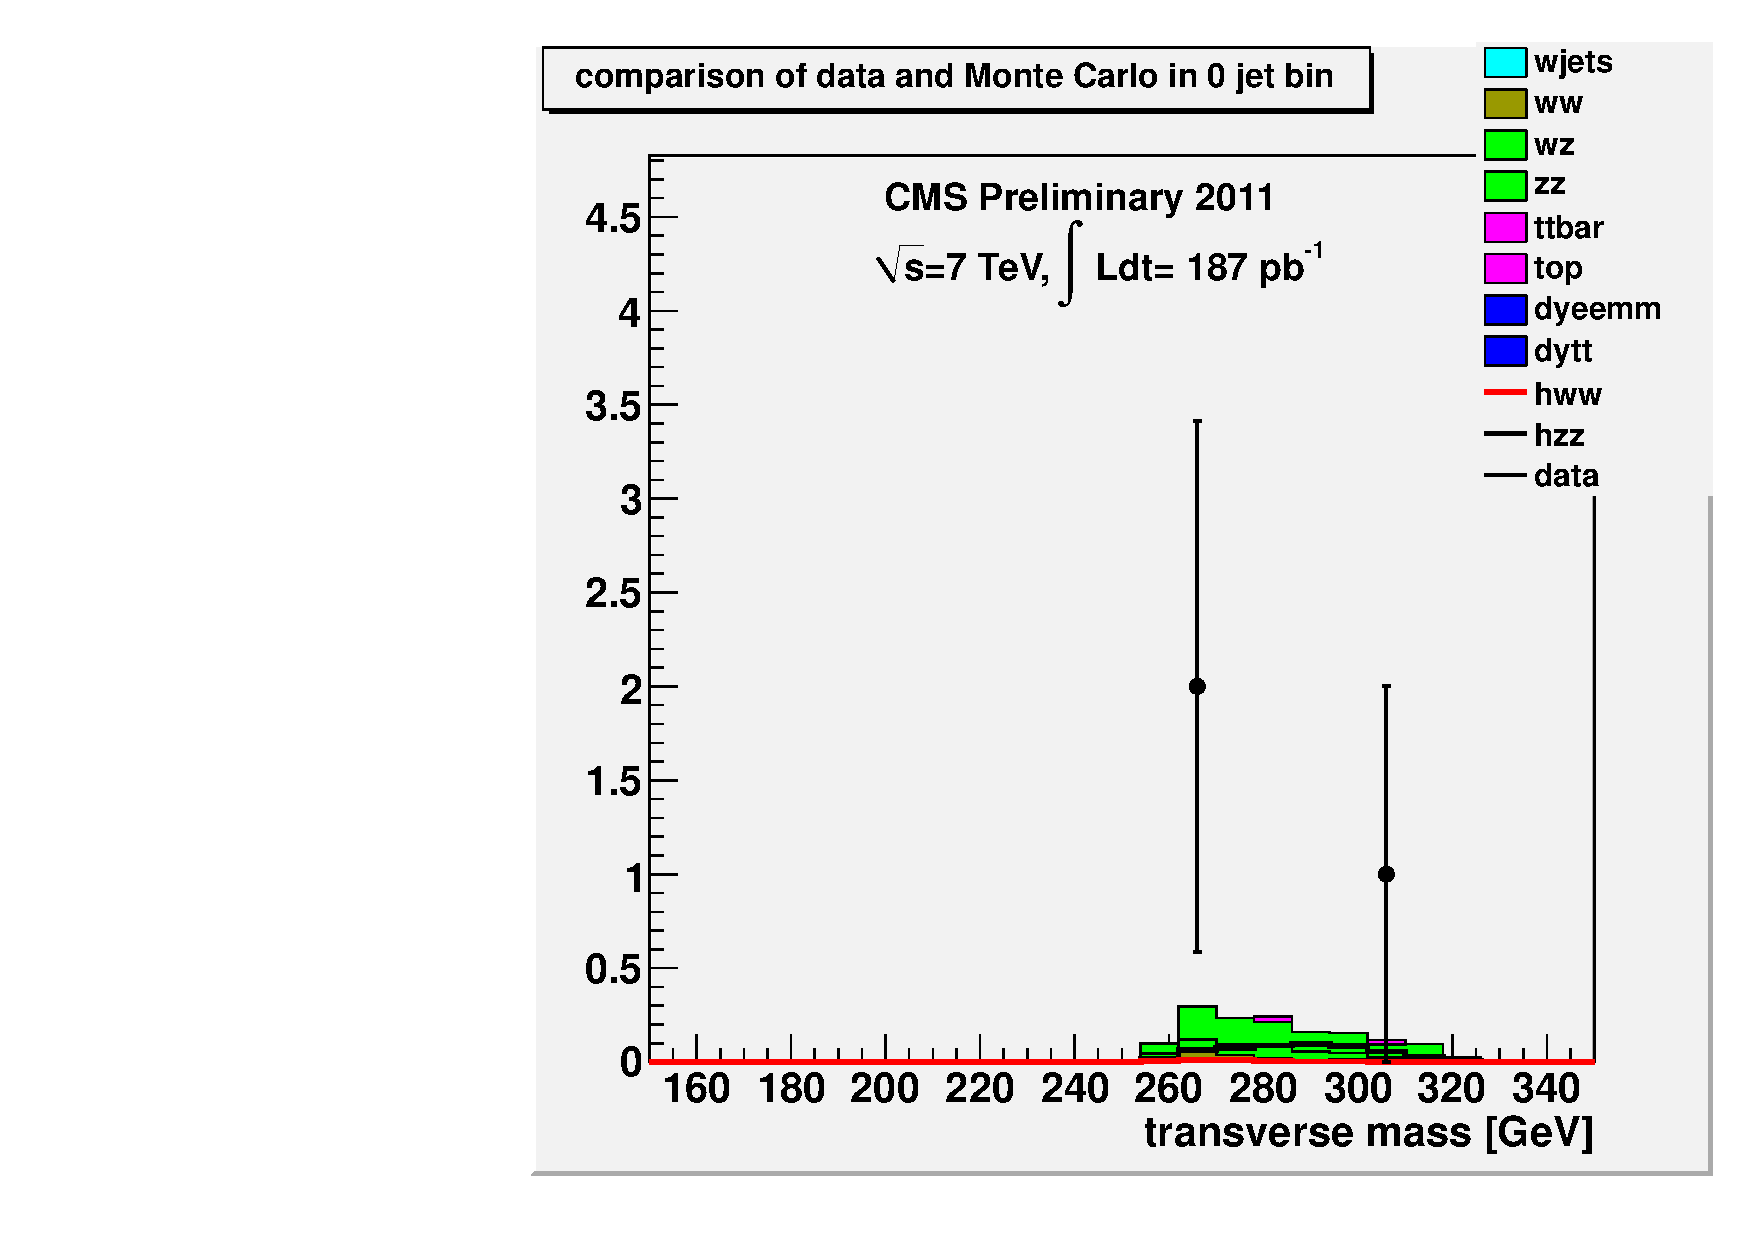
\includegraphics[width=.45\textwidth]{figures/fullselection_0jets_mt.pdf}}
\subfigure[1-Jet]{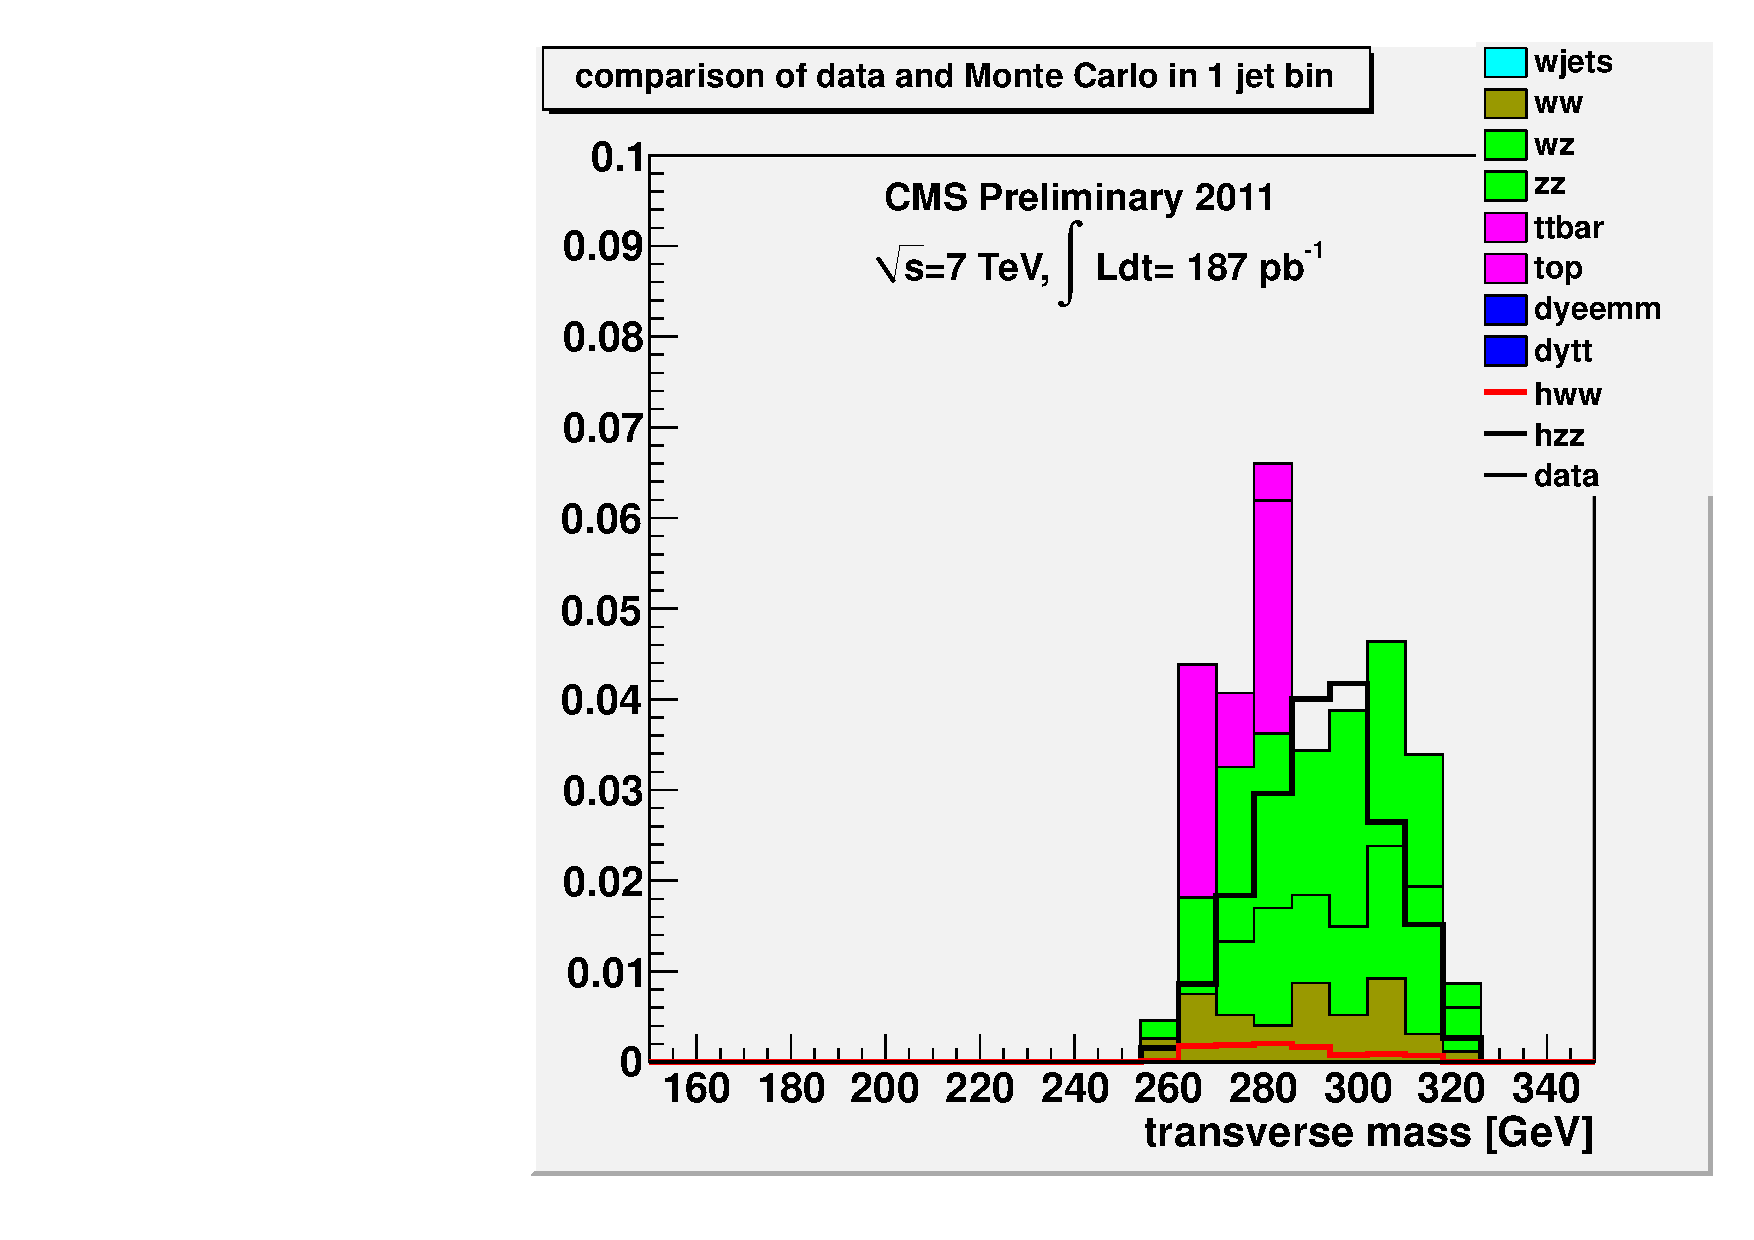
\includegraphics[width=.45\textwidth]{figures/fullselection_1jet_mt.pdf}}
\subfigure[$\geq$2 Jets]{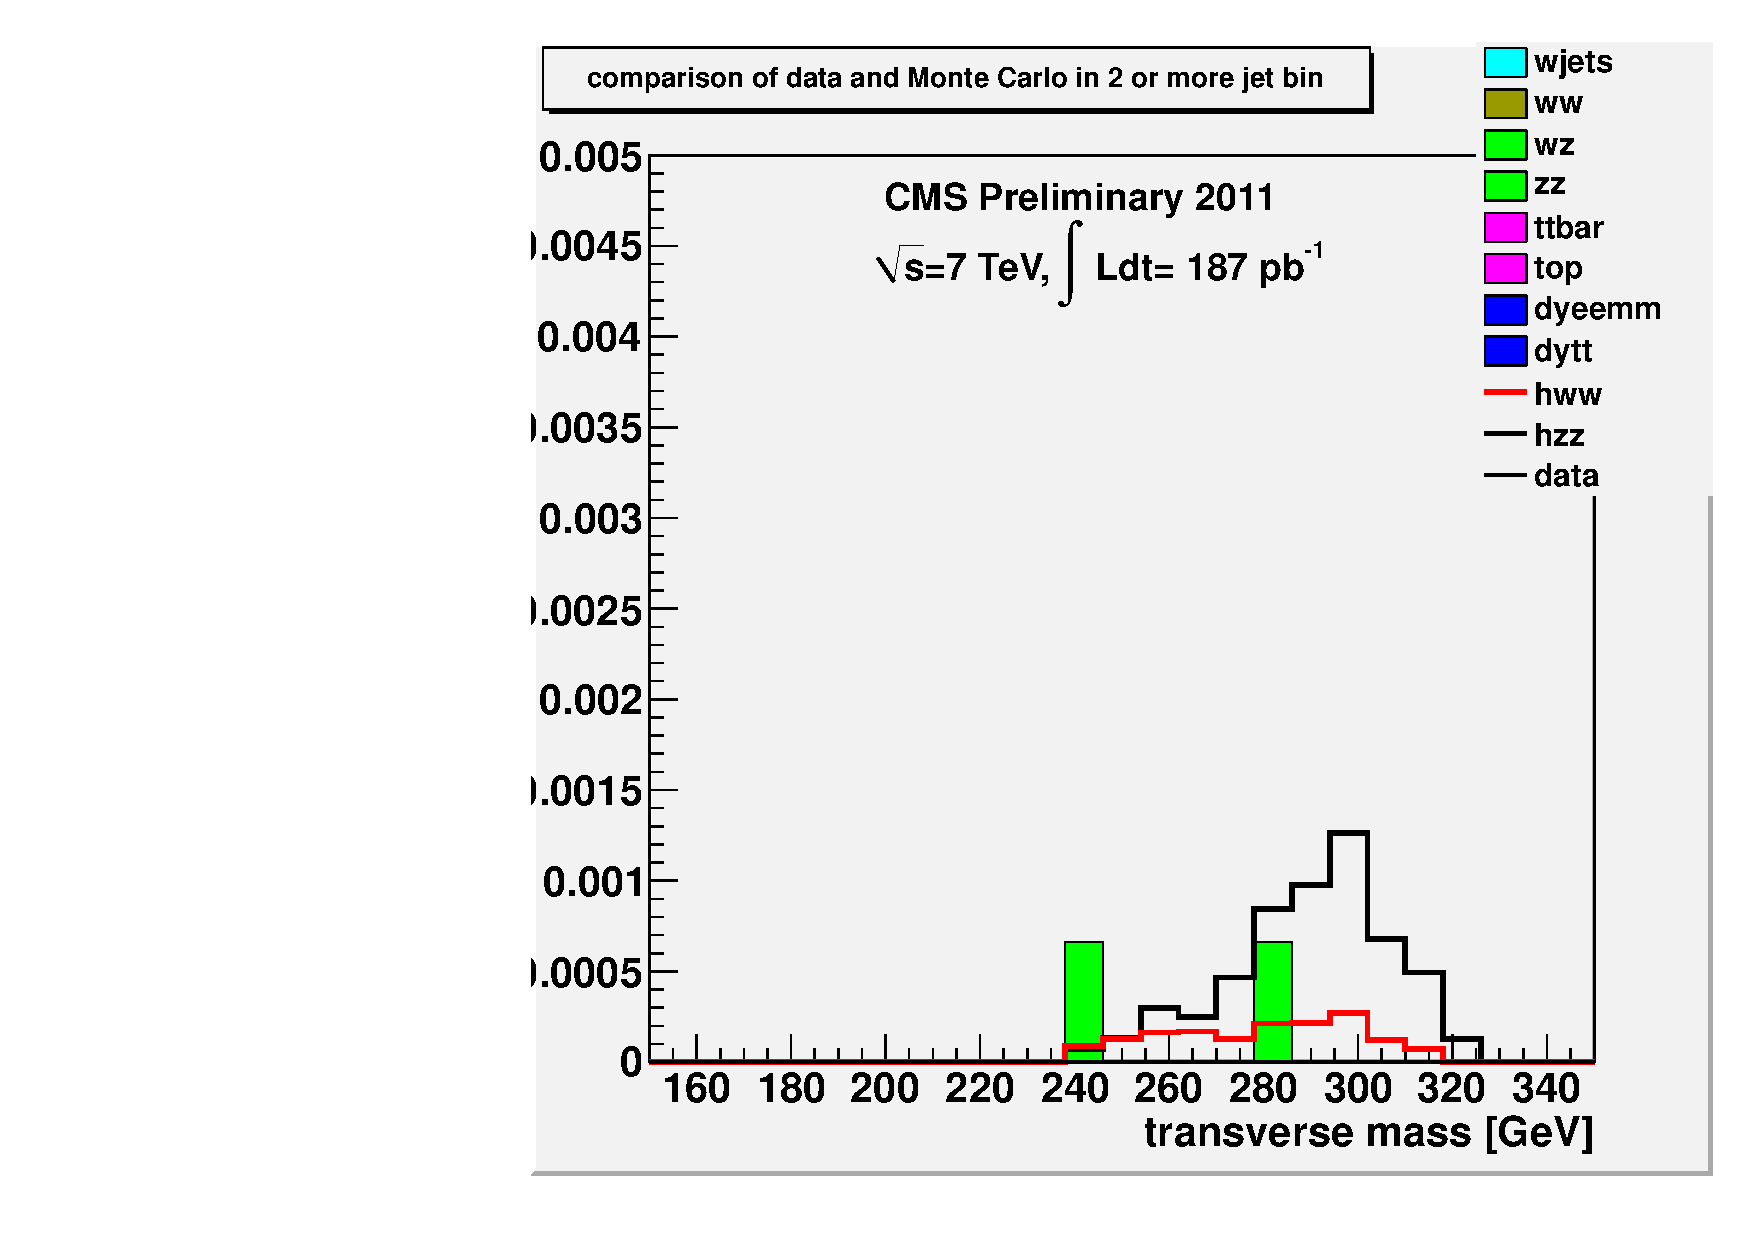
\includegraphics[width=.45\textwidth]{figures/fullselection_2jets_mt.pdf}}
\caption{The above figures display the background, higgs, and data yields as a function of the transverse mass after full 300 GeV selection. No efficiency scale factors were used, but pt reweighting was applied to the higgs MC.}
\end{center}
\end{figure}
%%%%%%%%

%%%%%%%%
\begin{figure}[!hbtp]
\begin{center}
\label{}
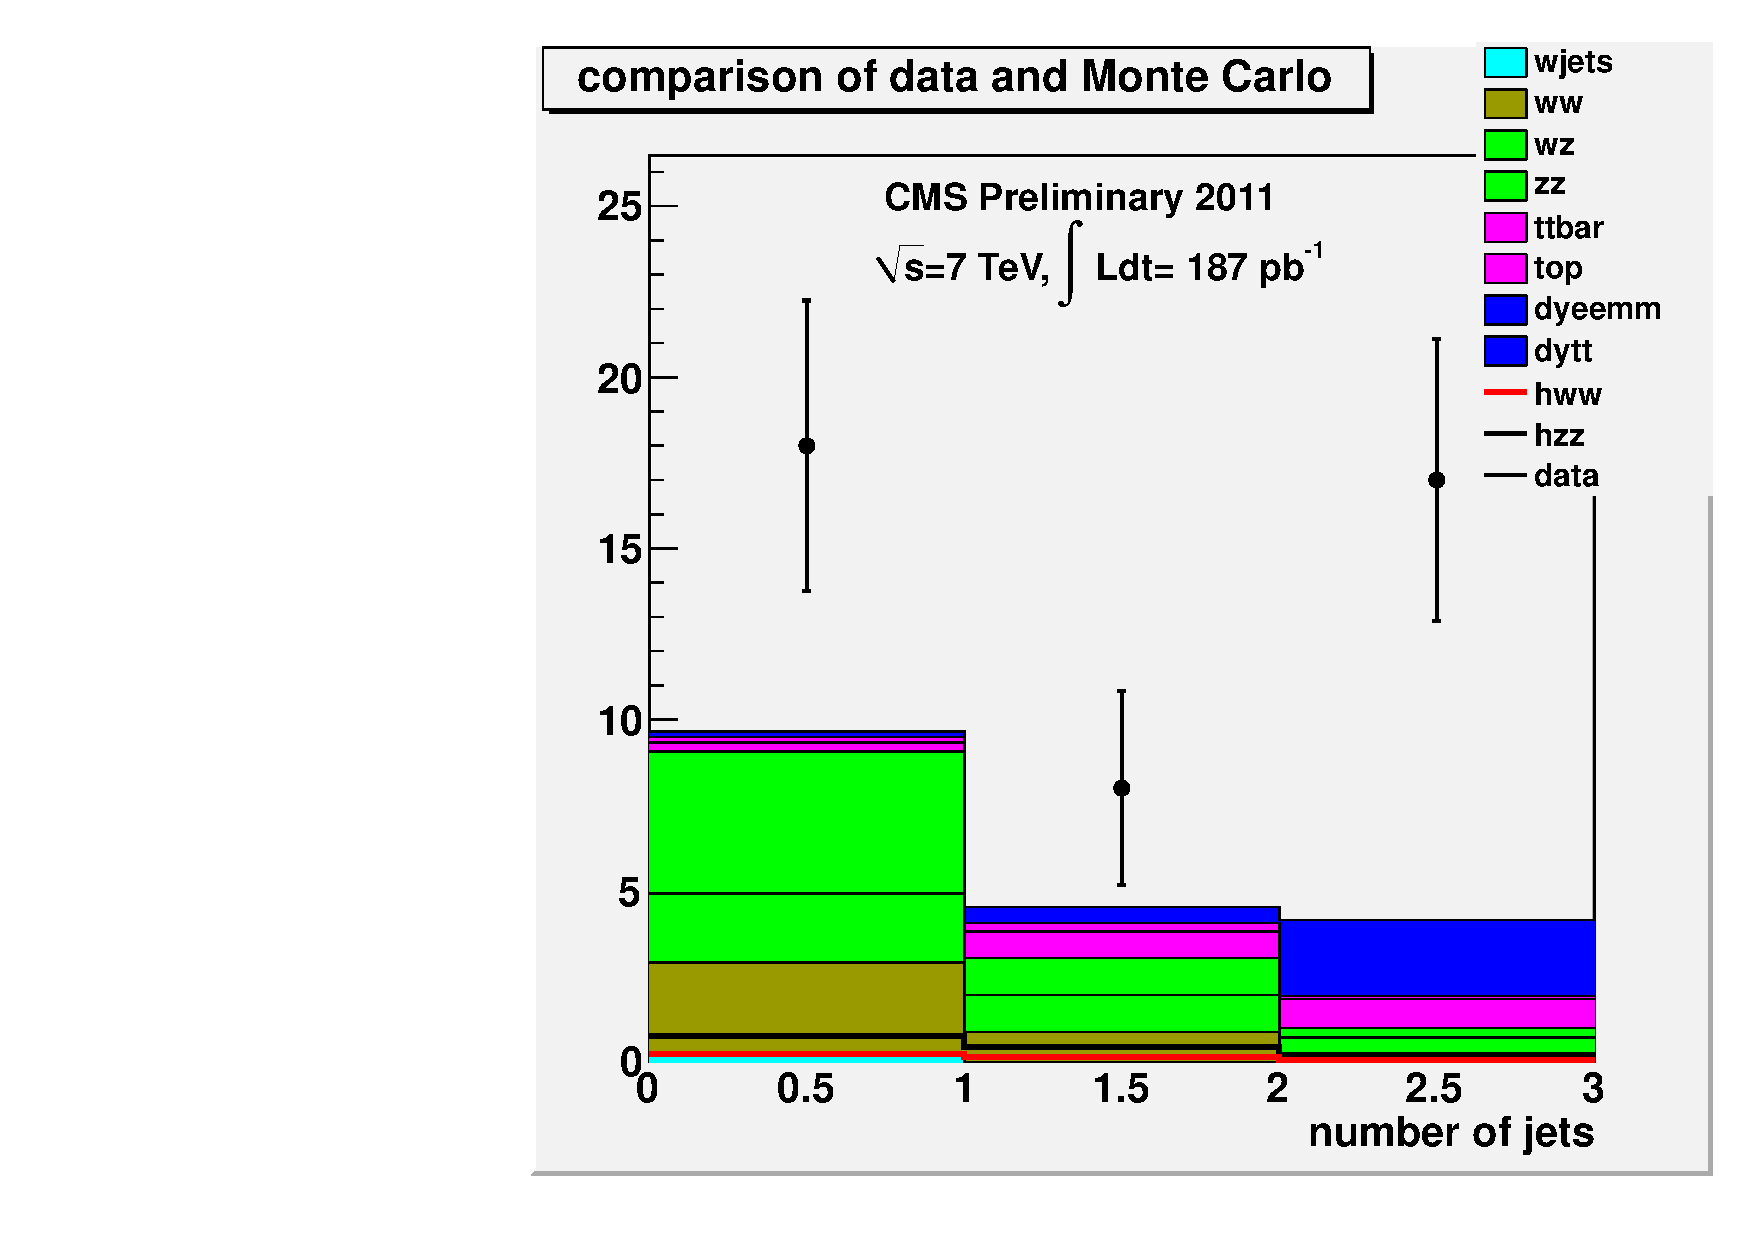
\includegraphics[width=.45\textwidth]{figures/preselection_njets.pdf}
\caption{The above figure displays the background, higgs, and data yields as a function of the number of jets after preselection. No efficiency scale factors were used, but pt reweighting was applied to the higgs MC.}
\end{center}
\end{figure}
%%%%%%%%

%%%%%%%%
\begin{figure}[!hbtp]
\begin{center}
\label{}
\subfigure[0-Jet]{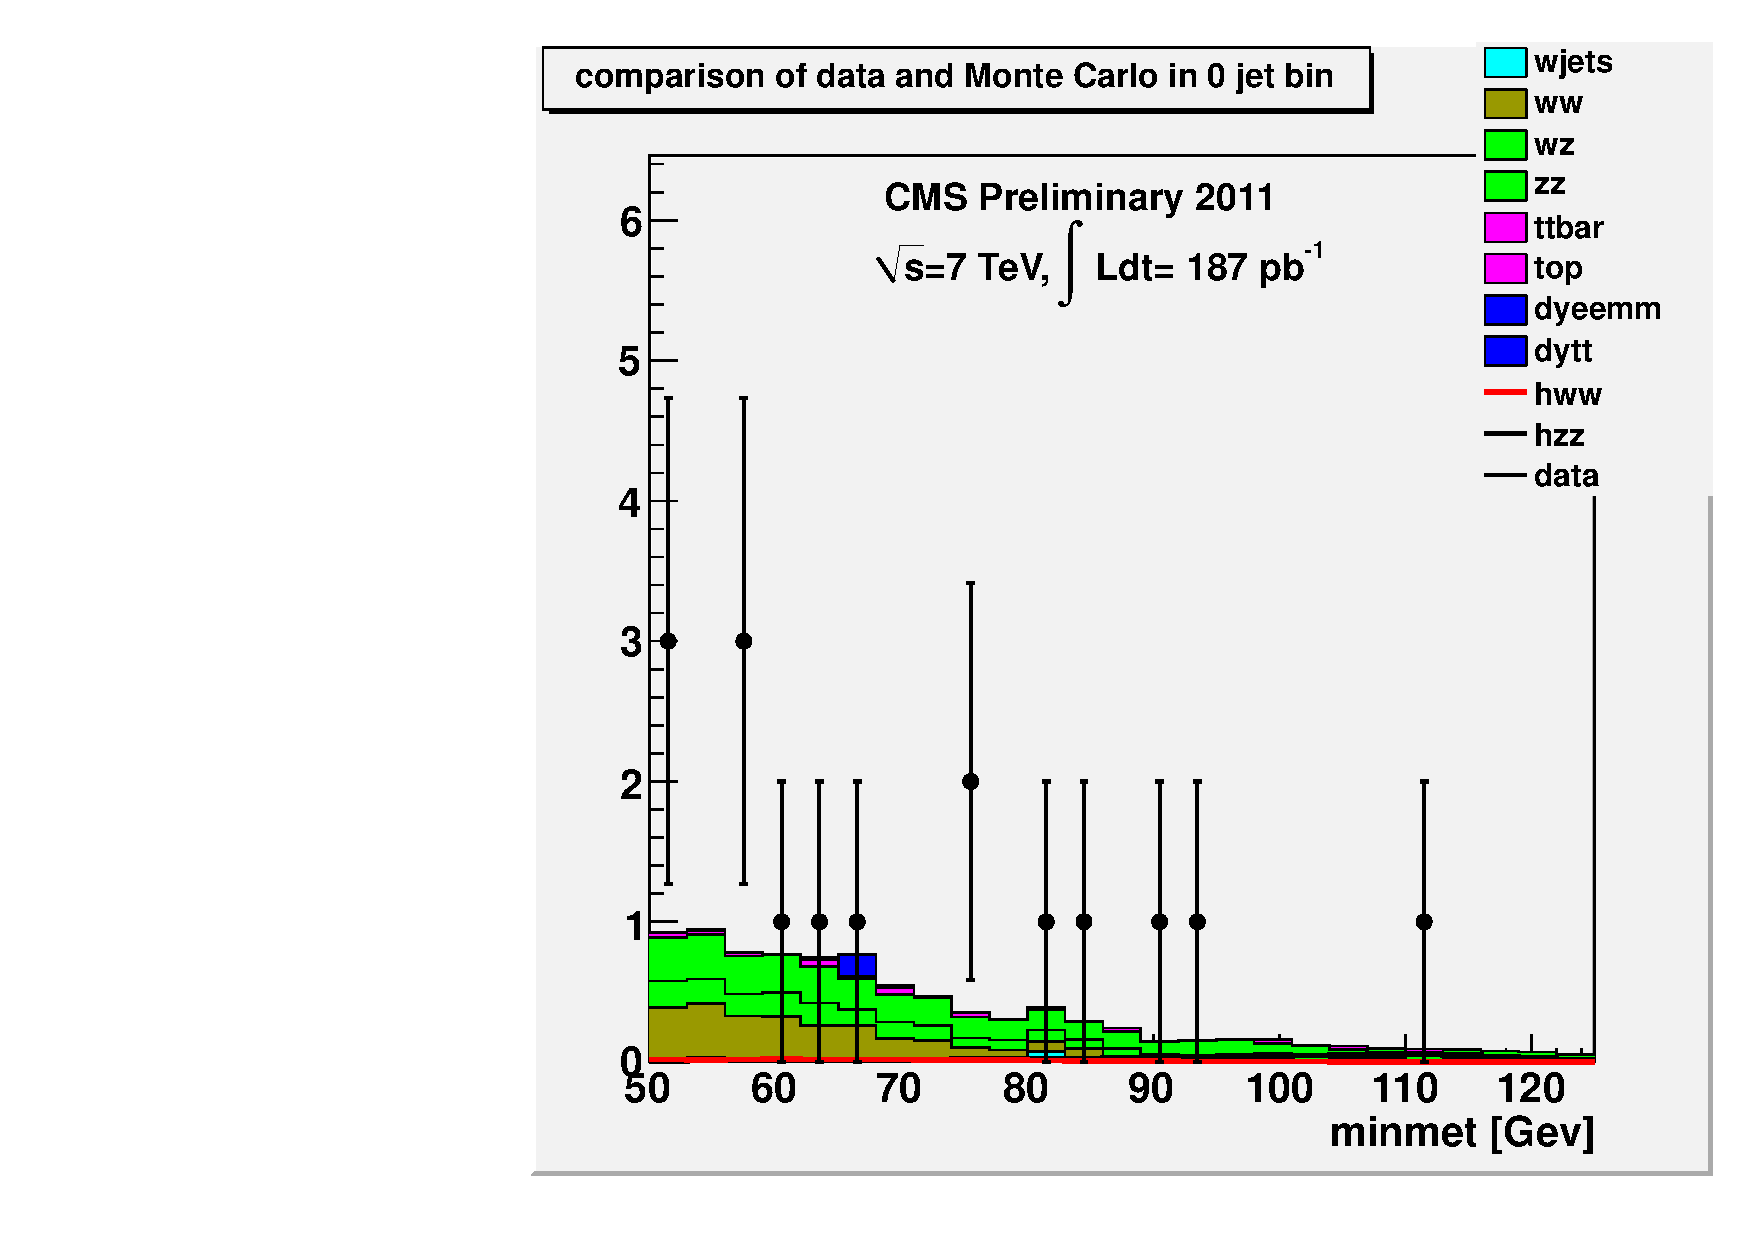
\includegraphics[width=.45\textwidth]{figures/preselection_0jets_minmet.pdf}}
\subfigure[1-Jet]{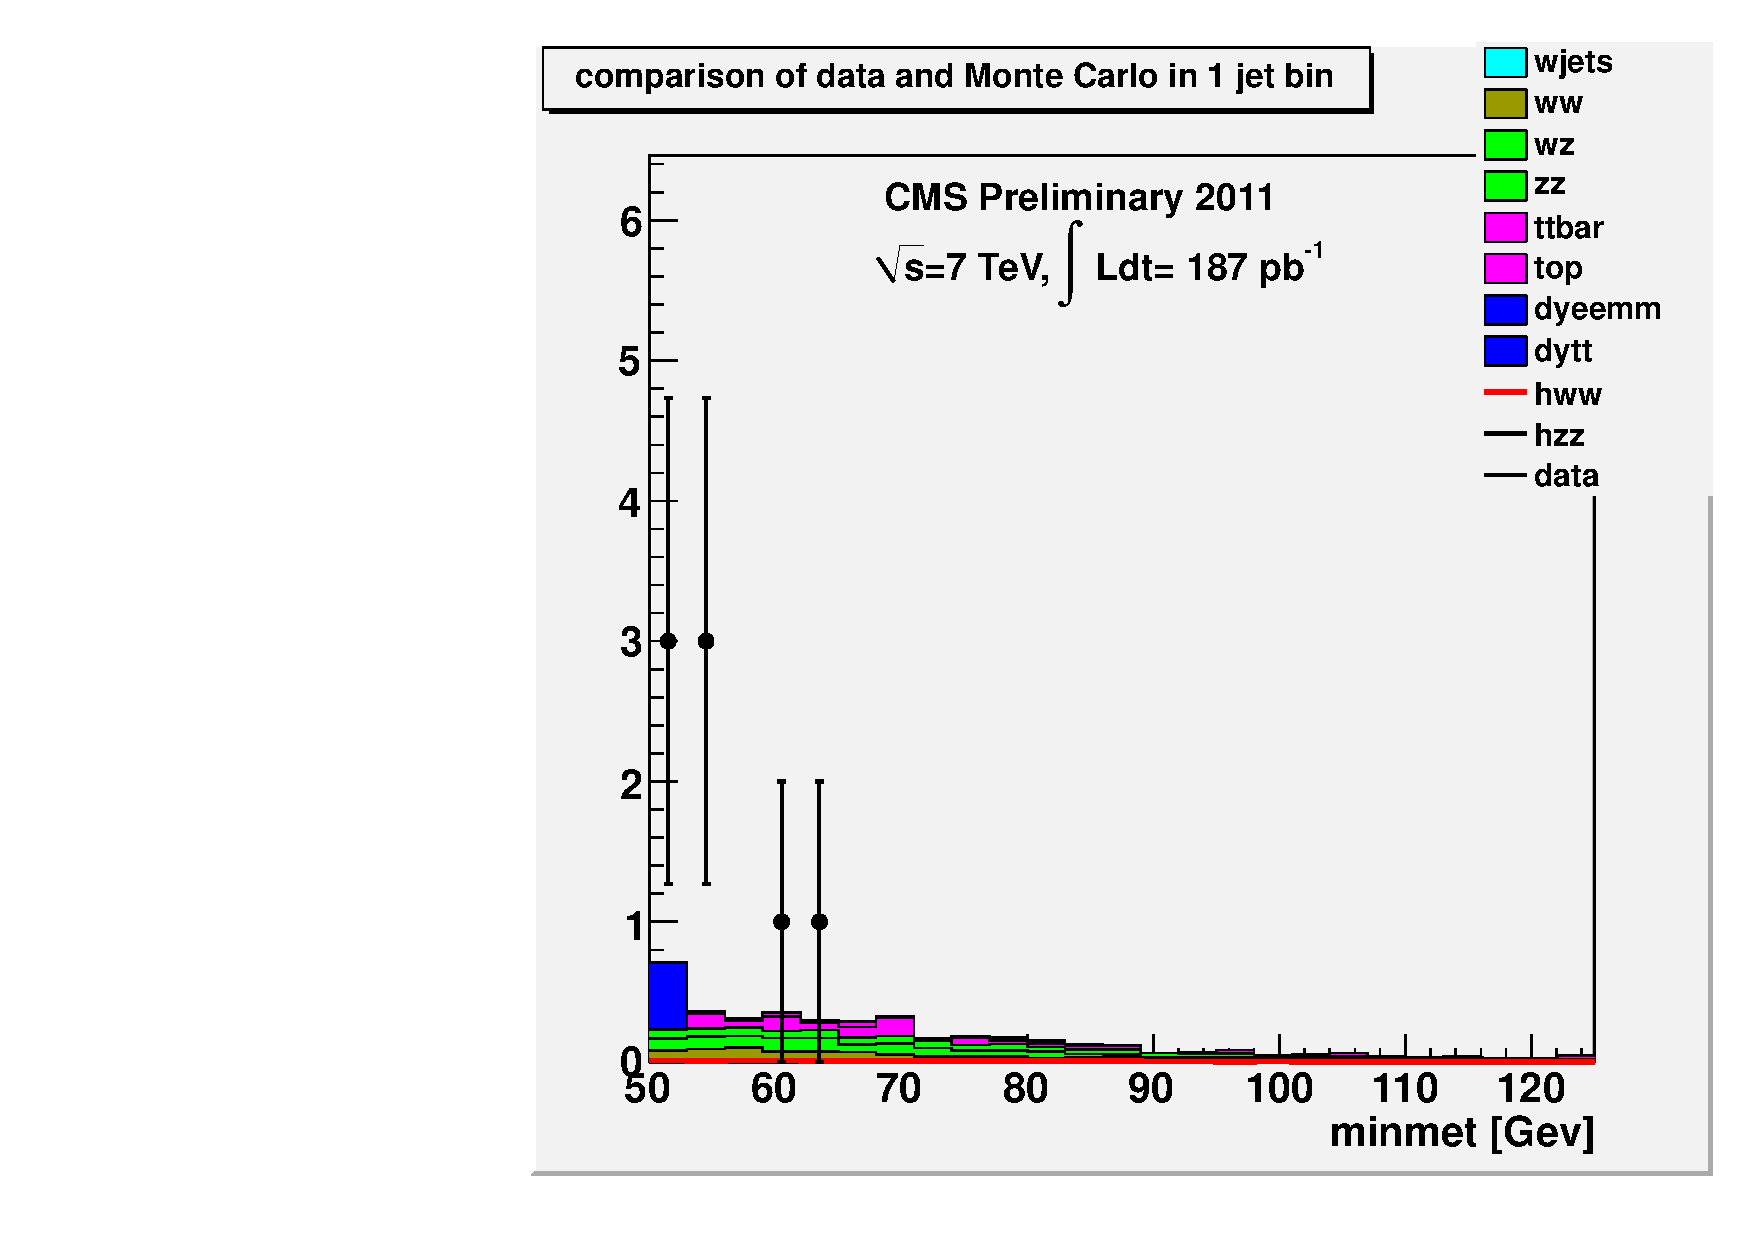
\includegraphics[width=.45\textwidth]{figures/preselection_1jet_minmet.pdf}}
\subfigure[$\geq$2 Jets]{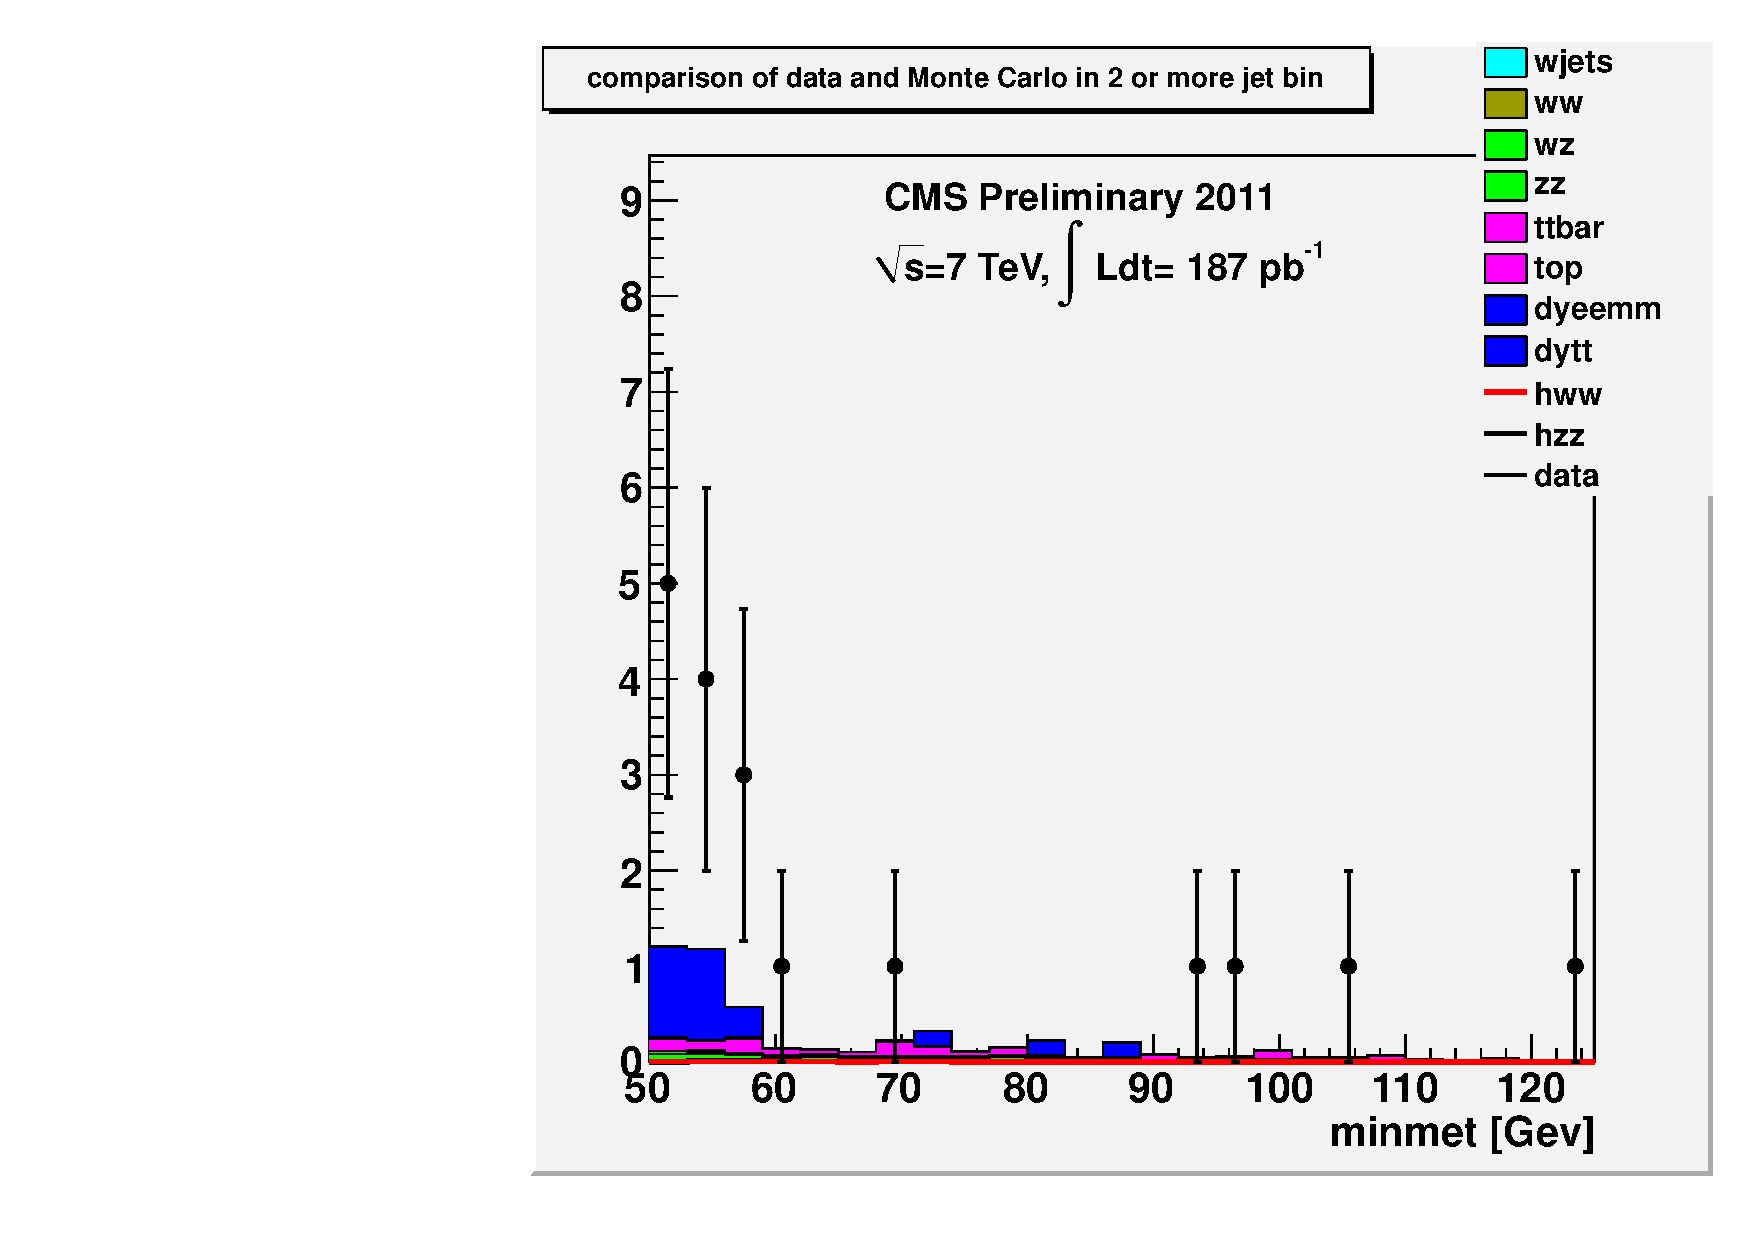
\includegraphics[width=.45\textwidth]{figures/preselection_2jets_minmet.pdf}}
\caption{The above figures display the background, higgs, and data yields as a function of min(met,tracker met) after preselection. No efficiency scale factors were used, but pt reweighting was applied to the higgs MC.}
\end{center}
\end{figure}
%%%%%%%%

%%%%%%%%
\begin{figure}[!hbtp]
\begin{center}
\label{}
\subfigure[0-Jet]{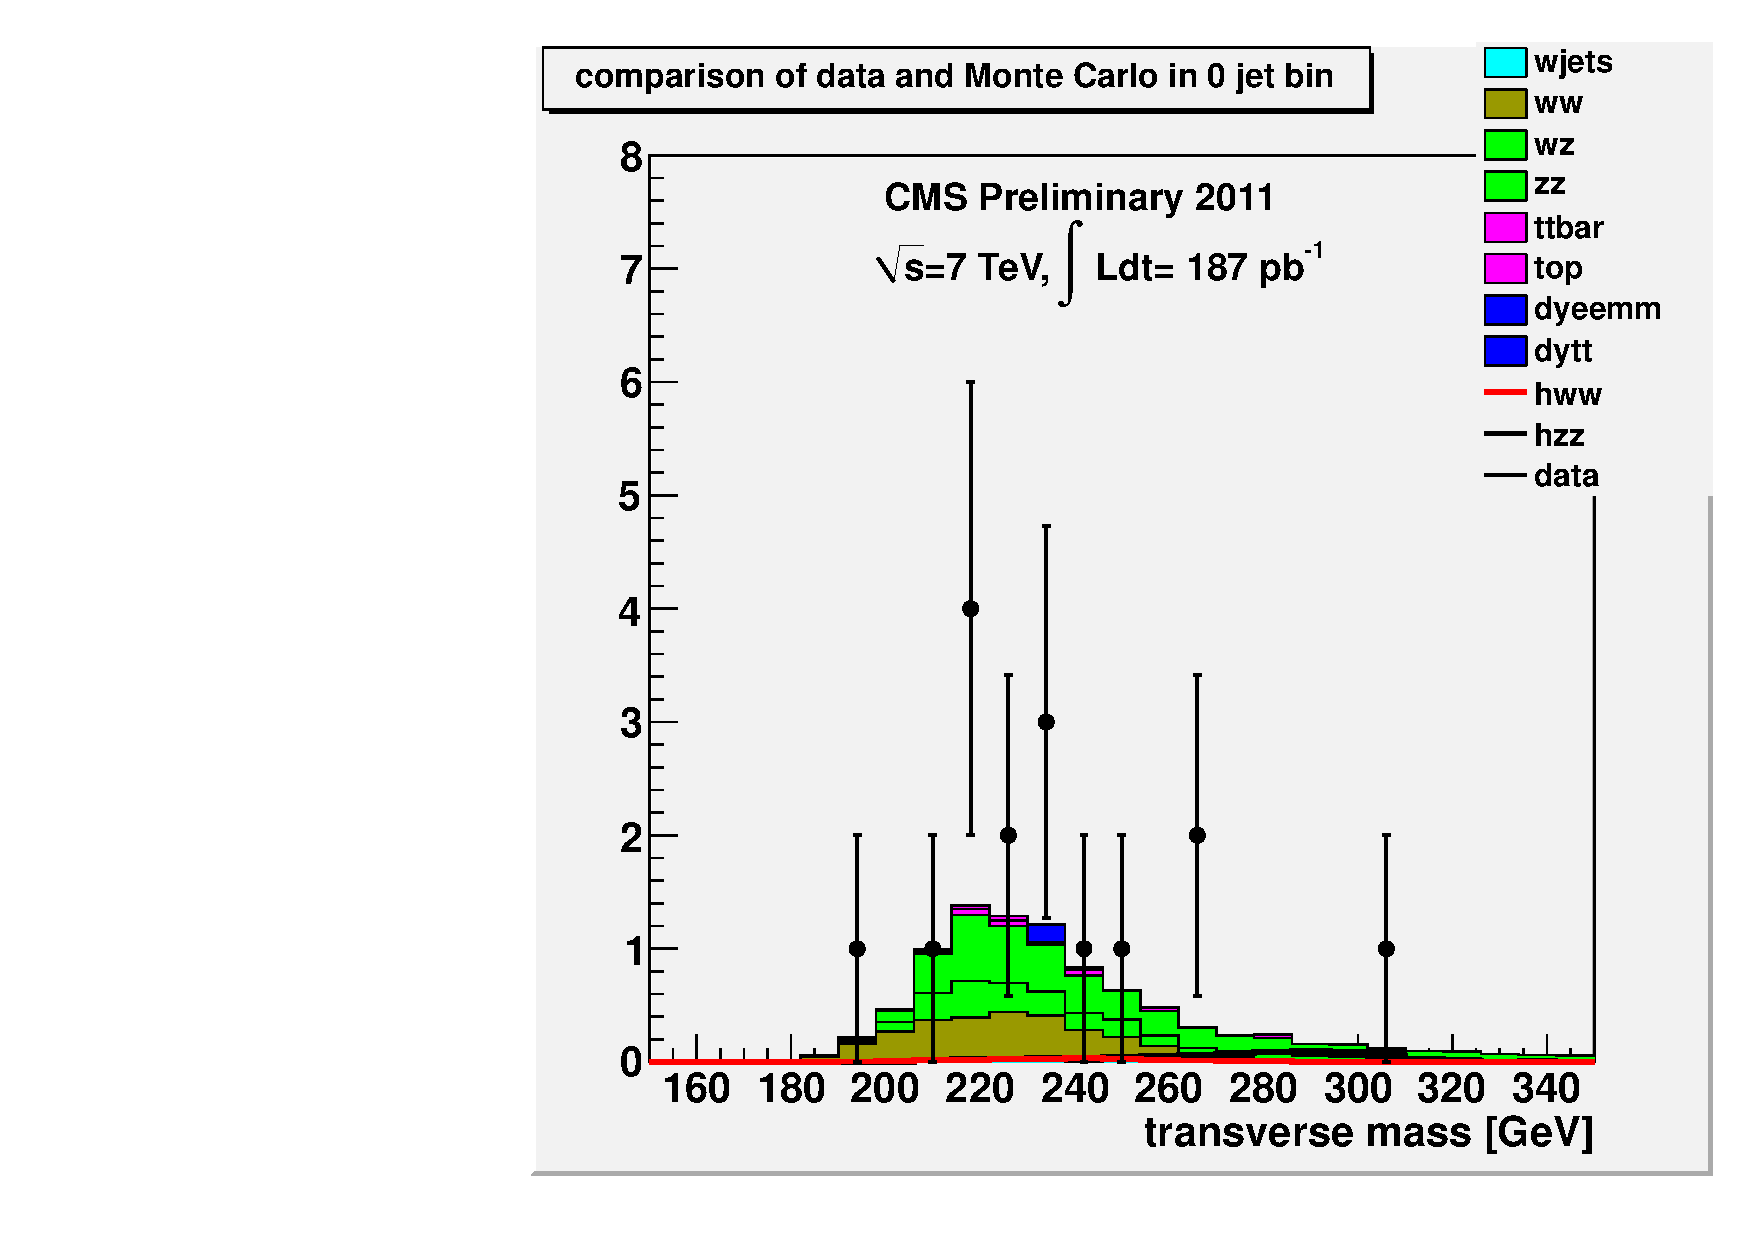
\includegraphics[width=.45\textwidth]{figures/preselection_0jets_mt.pdf}}
\subfigure[1-Jet]{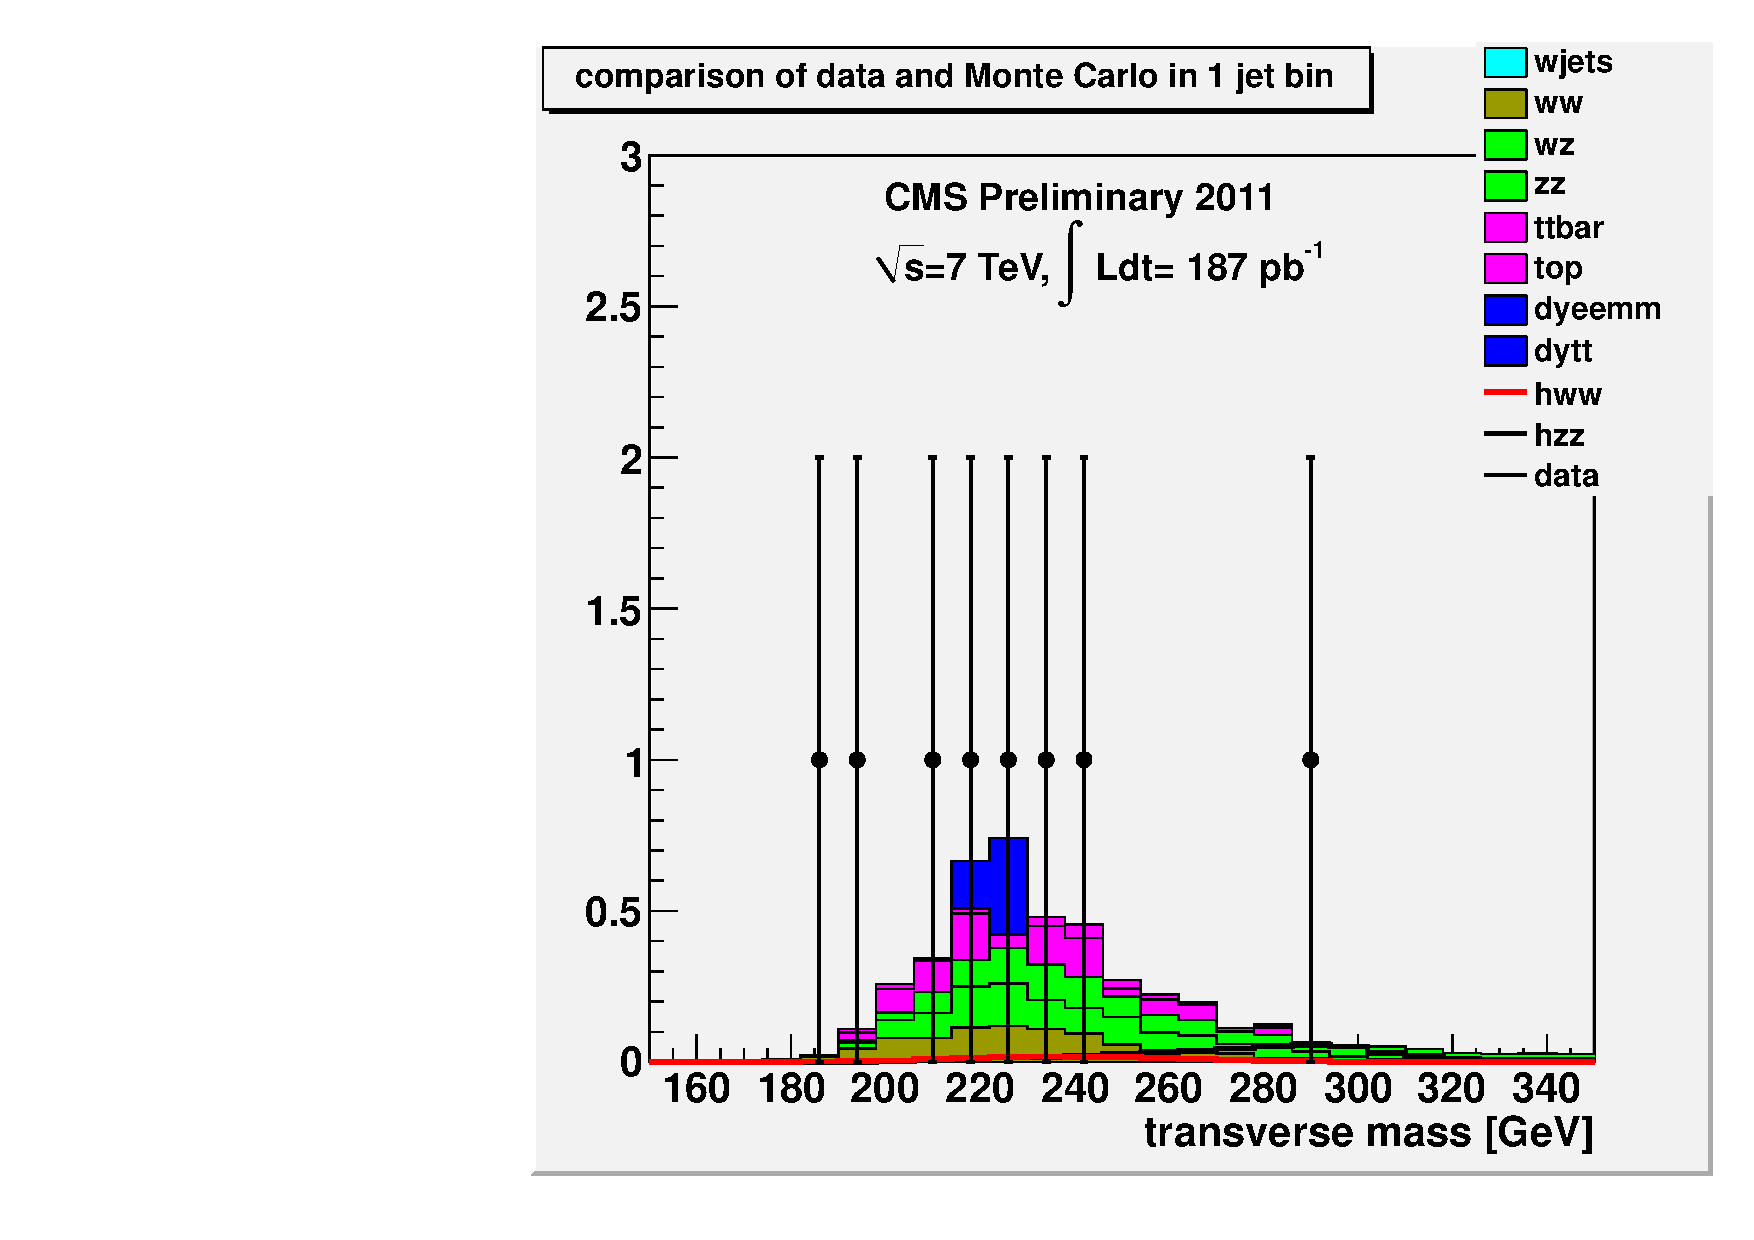
\includegraphics[width=.45\textwidth]{figures/preselection_1jet_mt.pdf}}
\subfigure[$\geq$2 Jets]{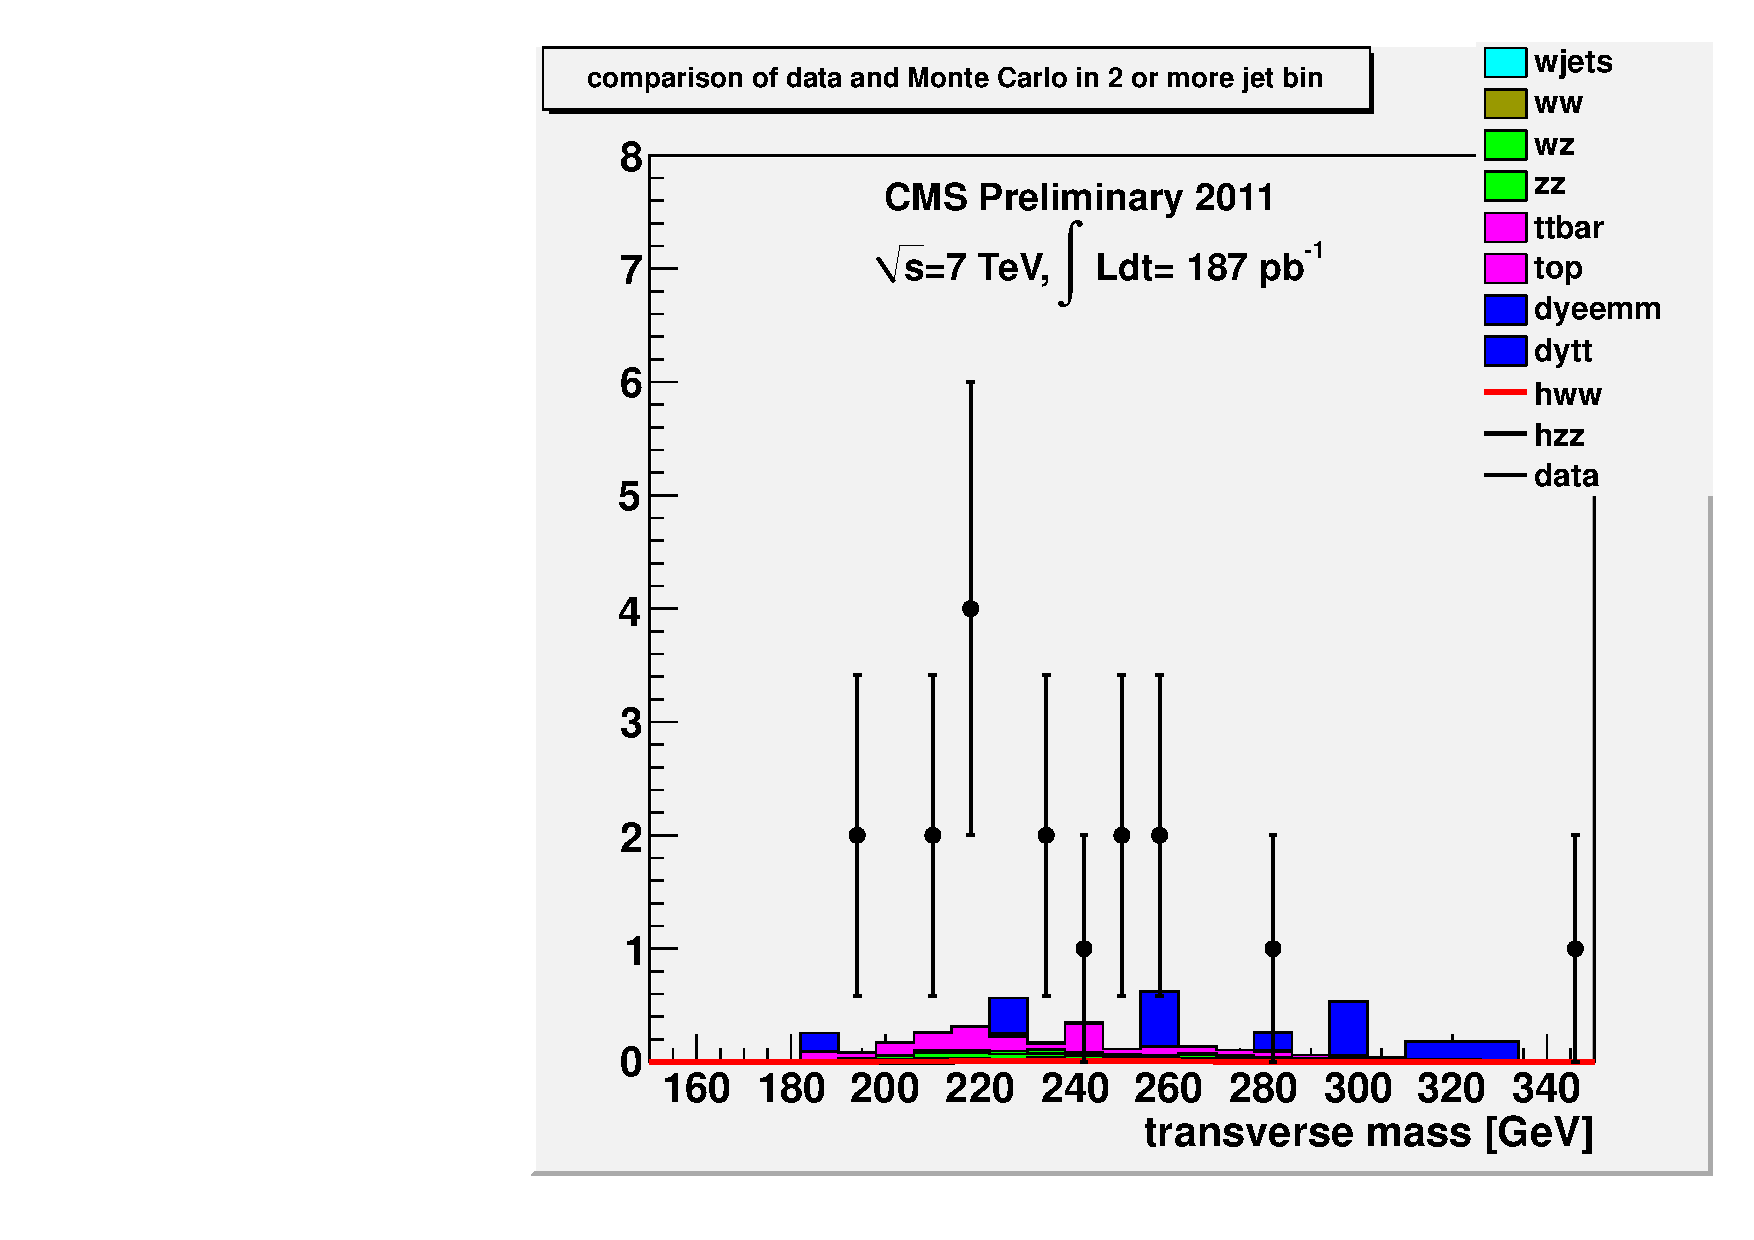
\includegraphics[width=.45\textwidth]{figures/preselection_2jets_mt.pdf}}
\caption{The above figures display the background, higgs, and data yields as a function of the transverse mass after preselection. No efficiency scale factors were used, but pt reweighting was applied to the higgs MC.}
\end{center}
\end{figure}
%%%%%%%%